
%<<setup-child, include = FALSE>>=
%library(knitr)
%library(ggplot2)
%library(microbenchmark)
%set_parent("../style/preamble.Rnw")
%@

\input{../../2021/style/preamble4tex}
% dependencies: amsmath, amssymb, dsfont
% math spaces
\ifdefined\N
\renewcommand{\N}{\mathds{N}} % N, naturals
\else \newcommand{\N}{\mathds{N}} \fi
\newcommand{\Z}{\mathds{Z}} % Z, integers
\newcommand{\Q}{\mathds{Q}} % Q, rationals
\newcommand{\R}{\mathds{R}} % R, reals
\ifdefined\C
\renewcommand{\C}{\mathds{C}} % C, complex
\else \newcommand{\C}{\mathds{C}} \fi
\newcommand{\continuous}{\mathcal{C}} % C, space of continuous functions
\newcommand{\M}{\mathcal{M}} % machine numbers
\newcommand{\epsm}{\epsilon_m} % maximum error

% counting / finite sets
\newcommand{\setzo}{\{0, 1\}} % set 0, 1
\newcommand{\setmp}{\{-1, +1\}} % set -1, 1
\newcommand{\unitint}{[0, 1]} % unit interval

% basic math stuff
\newcommand{\xt}{\tilde x} % x tilde
\newcommand{\argmin}{\mathop{\mathrm{arg\,min}}} % argmin
\newcommand{\argmax}{\mathop{\mathrm{arg\,max}}} % argmax
\newcommand{\argminlim}{\argmin\limits} % argmin with limits
\newcommand{\argmaxlim}{\argmax\limits} % argmax with limits
\newcommand{\sign}{\operatorname{sign}} % sign, signum
\newcommand{\I}{\mathbb{I}} % I, indicator
\newcommand{\order}{\mathcal{O}} % O, order
\newcommand{\bigO}{\mathcal{O}} % Big-O Landau
\newcommand{\littleo}{{o}} % Little-o Landau
\newcommand{\pd}[2]{\frac{\partial{#1}}{\partial #2}} % partial derivative
\newcommand{\floorlr}[1]{\left\lfloor #1 \right\rfloor} % floor
\newcommand{\ceillr}[1]{\left\lceil #1 \right\rceil} % ceiling
\newcommand{\indep}{\perp \!\!\! \perp} % independence symbol

% sums and products
\newcommand{\sumin}{\sum\limits_{i=1}^n} % summation from i=1 to n
\newcommand{\sumim}{\sum\limits_{i=1}^m} % summation from i=1 to m
\newcommand{\sumjn}{\sum\limits_{j=1}^n} % summation from j=1 to p
\newcommand{\sumjp}{\sum\limits_{j=1}^p} % summation from j=1 to p
\newcommand{\sumik}{\sum\limits_{i=1}^k} % summation from i=1 to k
\newcommand{\sumkg}{\sum\limits_{k=1}^g} % summation from k=1 to g
\newcommand{\sumjg}{\sum\limits_{j=1}^g} % summation from j=1 to g
\newcommand{\summM}{\sum\limits_{m=1}^M} % summation from m=1 to M
\newcommand{\meanin}{\frac{1}{n} \sum\limits_{i=1}^n} % mean from i=1 to n
\newcommand{\meanim}{\frac{1}{m} \sum\limits_{i=1}^m} % mean from i=1 to n
\newcommand{\meankg}{\frac{1}{g} \sum\limits_{k=1}^g} % mean from k=1 to g
\newcommand{\meanmM}{\frac{1}{M} \sum\limits_{m=1}^M} % mean from m=1 to M
\newcommand{\prodin}{\prod\limits_{i=1}^n} % product from i=1 to n
\newcommand{\prodkg}{\prod\limits_{k=1}^g} % product from k=1 to g
\newcommand{\prodjp}{\prod\limits_{j=1}^p} % product from j=1 to p

% linear algebra
\newcommand{\one}{\bm{1}} % 1, unitvector
\newcommand{\zero}{\mathbf{0}} % 0-vector
\newcommand{\id}{\bm{I}} % I, identity
\newcommand{\diag}{\operatorname{diag}} % diag, diagonal
\newcommand{\trace}{\operatorname{tr}} % tr, trace
\newcommand{\spn}{\operatorname{span}} % span
\newcommand{\scp}[2]{\left\langle #1, #2 \right\rangle} % <.,.>, scalarproduct
\newcommand{\mat}[1]{\begin{pmatrix} #1 \end{pmatrix}} % short pmatrix command
\newcommand{\Amat}{\mathbf{A}} % matrix A
\newcommand{\Deltab}{\mathbf{\Delta}} % error term for vectors

% basic probability + stats
\renewcommand{\P}{\mathds{P}} % P, probability
\newcommand{\E}{\mathds{E}} % E, expectation
\newcommand{\var}{\mathsf{Var}} % Var, variance
\newcommand{\cov}{\mathsf{Cov}} % Cov, covariance
\newcommand{\corr}{\mathsf{Corr}} % Corr, correlation
\newcommand{\normal}{\mathcal{N}} % N of the normal distribution
\newcommand{\iid}{\overset{i.i.d}{\sim}} % dist with i.i.d superscript
\newcommand{\distas}[1]{\overset{#1}{\sim}} % ... is distributed as ...


\begin{document}

\lecturechapter{6}{(Adaptive) Rejection Sampling}
\lecture{CIM1 Statistical Computation}


\begin{vbframe}{Rejection Sampling}
\begin{itemize}
\item Aim: Generate random numbers $X$ from a distribution with density $f_X(x)$.
\item Idea: Draw $Y$ from distribution with density $f_Y(y)$ (Proposal density) instead; \\
 there must be a $\beta$ with $0 < \beta < 1$ such that $\beta f_X(x) \leq f_Y(x)$ for all
  $x \in \mbox{supp}(X)$.
\item Accept $Y$ as a random number from $f_X(x)$ with probability
  $$
  \alpha = \alpha(Y) = \beta \cdot \frac{f_X(Y)}{f_Y(Y)}
  $$
\end{itemize}

\framebreak


\begin{center}
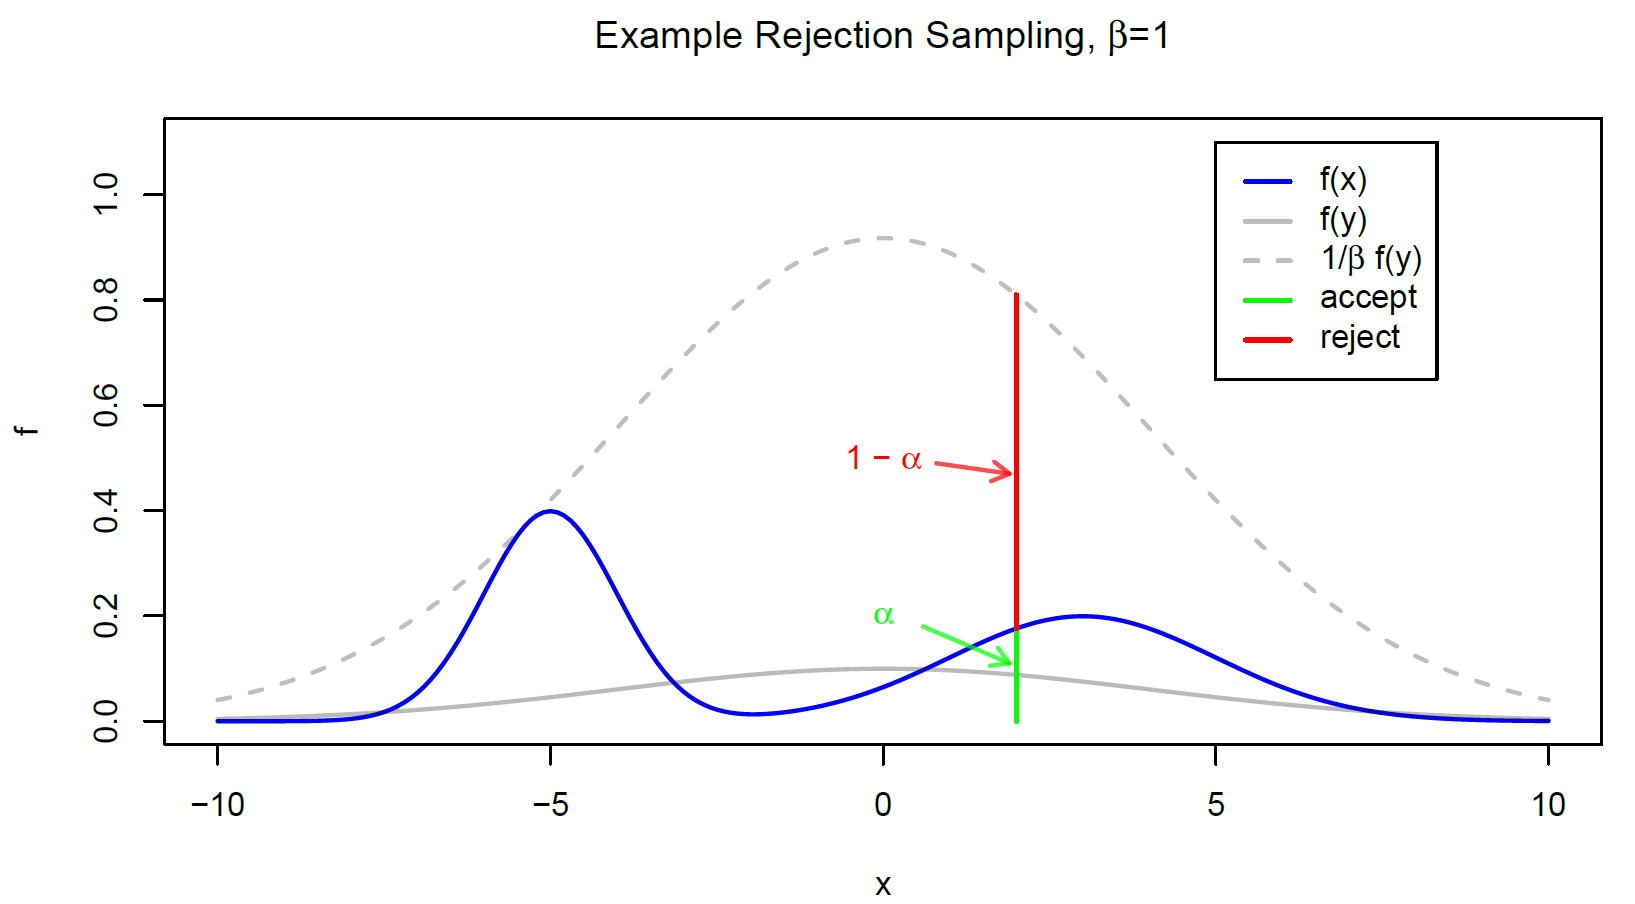
\includegraphics[width =0.8\textwidth]{figure_man/rejection.png}
\end{center}

%<<echo=FALSE>>=

%x = seq(-10, 10, .1)
%f_x = dnorm(x, 3, 2) + dnorm(x, -5, 1)
%f_y = dnorm(x, 0, 4)

%b = max(f_x / f_y)^-1

%env = f_y/b
%#which(x == 2) # 121

%plot(x, env, type = "l", col = "gray", lty = 2, lwd = 2, ylab = "f", ylim = c(0,1.1), main = expression(paste("Example Rejection Sampling, ", beta, "=", 1)))
%lines(x, f_x, col = "blue", lwd = 2)
%lines(x, f_y, col = rgb(.1, .1, .1, .3), lwd = 2)
%segments(2,0,2,f_x[121], col = "green", lwd = 2)
%segments(2,f_x[121],2,env[121], col = "red", lwd = 2)
%legend(5, 1.1, legend = c("f(x)", "f(y)", expression(paste("1/", beta, " f(y)")), "accept", "reject"),
%              col = c("blue", "gray", "gray", "green", "red"),
%              lwd = 2,
%              lty = c(1,1,2,1,1),
%              seg.len = 1.5
%              )
%text(0, .5, labels = expression(paste("1 - ", alpha)), col = rgb(1,0,0,1))
%text(0, .2, labels = expression(alpha), col = rgb(0,1,0,1))
%arrows(.8, .49, 1.9, .47, col = rgb(1,0,0,.7), length = 0.1, lwd = 2)
%arrows(.6, .18, 1.9, .11, col = rgb(0,1,0,.7), length = 0.1, lwd = 2)
%@

\vspace*{-0.3cm}
\begin{footnotesize}
\textbf{Note:} In this plot $\alpha$ is shown as a percentage of the \enquote{total distance}, so it does not refer to the y-axis in the plot.
\end{footnotesize}

\framebreak

\begin{algorithm}[H]
  \caption{Rejection Sampling}
  \begin{algorithmic}[1]
  \State{Initialization: $f_Y, f_X, \beta, N$ (number of RV needed)}
  \State{$i \leftarrow 0$}
  \While{$i \ne N$}
    \State{Create a random number $Y$ from $f_Y$ ($Y \sim f_Y$)}
    \State{Calculate
    $
    \alpha(Y) = \frac{\beta f_X(Y)}{ f_Y(Y)}
    $}
    \State{Create a random number $U \sim \text{U}(0, 1)$ independent of $Y$}
    \If{$U \leq \alpha(Y)$}
      \State{Accept $Y$}
      \State{$i \leftarrow i + $1}
    \Else
      \State{Reject $Y$}
    \EndIf
  \EndWhile
  \end{algorithmic}
\end{algorithm}

% \framebreak
% \begin{itemize}
% \item[] \code{REPEAT}
%   \medskip
%   \begin{enumerate}
%   \item Erzeuge eine Zufallszahl $Y$ aus $f_Y$, also $Y \sim f_Y$.
%   \item Berechne
%     $$
%     \alpha(Y) = \frac{\beta f_X(Y)}{ f_Y(Y)}.
%     $$
%   \item Erzeuge eine von $Y$ unabhängige Zufallszahl $U$ aus
%     einer Gleichverteilung auf $[0,1]$: $U \sim U[0,1]$.
%   \end{enumerate}
%   \medskip
% \item[] \code{UNTIL} $U \leq \alpha(Y)$
% \item[] \code{RETURN} $Y$
% \end{itemize}
\end{vbframe}


\begin{vbframe}{Proof: Rejection Sampling}
$$ P(Y\le x \mid U\le \alpha(Y)) = \frac{P(Y\le x, U\le \alpha(Y))}{P(U\le\alpha(Y))}
$$
$Y, U$ independent $\Rightarrow$ common density $f(y,u)=f_Y(y)\cdot 1=f_Y(y)$
\begin{align*}
P(Y\le x, U\le\alpha(Y)) &= \int_{-\infty}^{x}\int_{0}^{\alpha(y)}f_Y(y)\,du\,dy
%\\
%&=\int_{-\infty}^{x}\int_{0}^{\alpha(y)}\,du f_Y(y)\,dy\\
%&
=\int_{-\infty}^{x}\alpha(y) f_Y(y)\,dy\\
&=\int_{-\infty}^{x}\beta\frac{f_X(y)}{f_Y(y)} f_Y(y)\,dy
=\beta\int_{-\infty}^{x}f_X(y)\,dy\\
\end{align*}
$$P(U\le\alpha(Y)) = P(Y\le\infty,U\le\alpha(Y))
                 = \beta\int_{-\infty}^{\infty}f_X(y)\,dy=\beta
$$

\framebreak

In summary we obtain exactly what was required
$$
P(Y\le x \mid U\le \alpha(Y)) = \int_{-\infty}^{x}f_X(y)\,dy.
$$
Choice of Y:\\
The closer $f_Y$ to $f_X$, the closer $\alpha$ to 1.\\
$\Rightarrow$ There is less rejection, hence it is faster.\\
\medskip
However, random variables of $Y$ should be generated as quickly as possible.\\
\medskip
\textbf{Note:} $\beta$ is the probability of $Y$ being accepted. The greater $\beta$, the better.\\
\medskip
$\beta$ itself is not needed in the algorithm (only $\alpha(Y)$).\\ $\Rightarrow$ calculation of normalization constants not always needed.
\end{vbframe}


\begin{vbframe}{Example: Normal distribution}
Only to illustrate Rejection Sampling!
Rejection Sampling from $\normal(0,1)$-distribution via
Cauchy distribution (therefore we have Inverse transform sampling):
    \begin{eqnarray*}
        f_X(x) & = & \frac{1}{\sqrt{2\,\pi}} \,
            \exp(-\frac{1}{2}x^2) \\
        f_Y(x) & = & \frac{1}{\pi} \cdot \frac{1}{1 + x^2}
    \end{eqnarray*}
    It is easy to show that $\beta = \inf\limits_y \frac{f_Y(y)}{f_X(y)}
    = \sqrt{\frac{e}{2\,\pi}} \approx 0.657$. \\
    The probability of acceptance $\alpha(Y)$ is
    \begin{eqnarray*}
    \alpha(Y) &=& \frac{\beta f_X(Y)}{ f_Y(Y)} \\
              &=&  \frac{\sqrt{e}}{2} \, (1 + y^2) \,
                    \exp(-\frac{1}{2}y^2).
    \end{eqnarray*}

\framebreak

\lz

\begin{center}
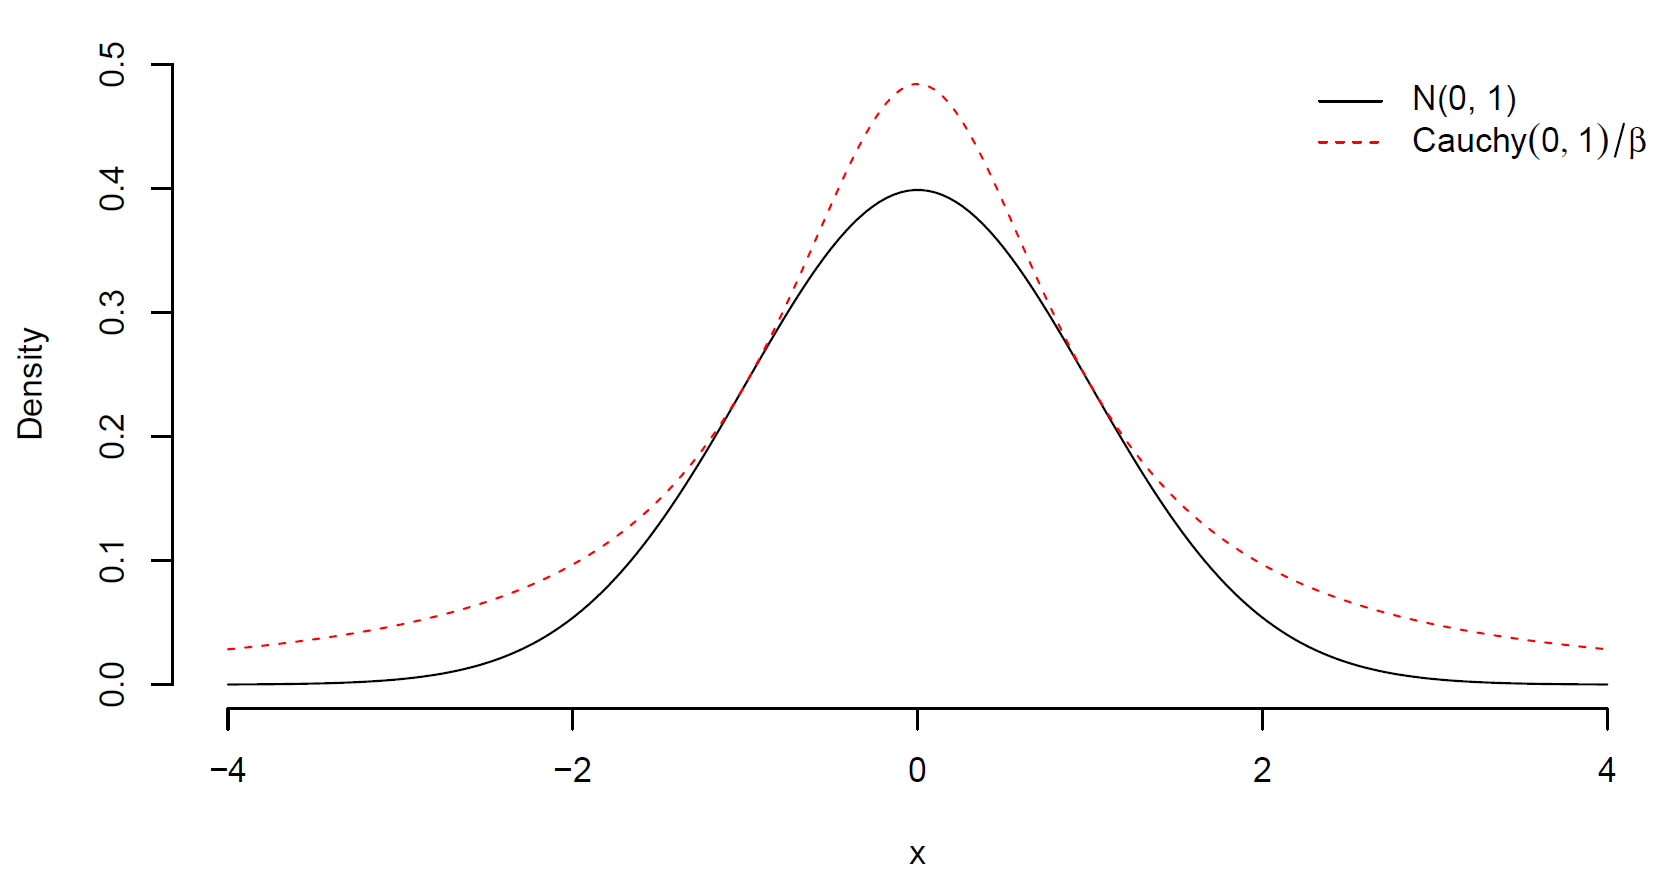
\includegraphics[width =0.9\textwidth]{figure_man/example.png}
\end{center}


%<<echo=FALSE>>=
%n = 200
%x = seq(-4, 4, length = n)
%dx = dnorm(x)
%dg = dcauchy(x) / 0.657
%plot(dx ~ x, type = "l", ylim = range(dx, dg),
%  lwd = 1, ylab = "Density", axes = FALSE)
%axis(1)
%axis(2)
%lines(dg ~ x, col = "red", lty = 2)
%legend("topright", c("N(0, 1)", expression(Cauchy(0, 1) / beta)), lwd = 1, col = c("black", "red"),
%  lty = c(1, 2), box.col = NA, bg = NA)
%@


\framebreak
\lz

\begin{center}
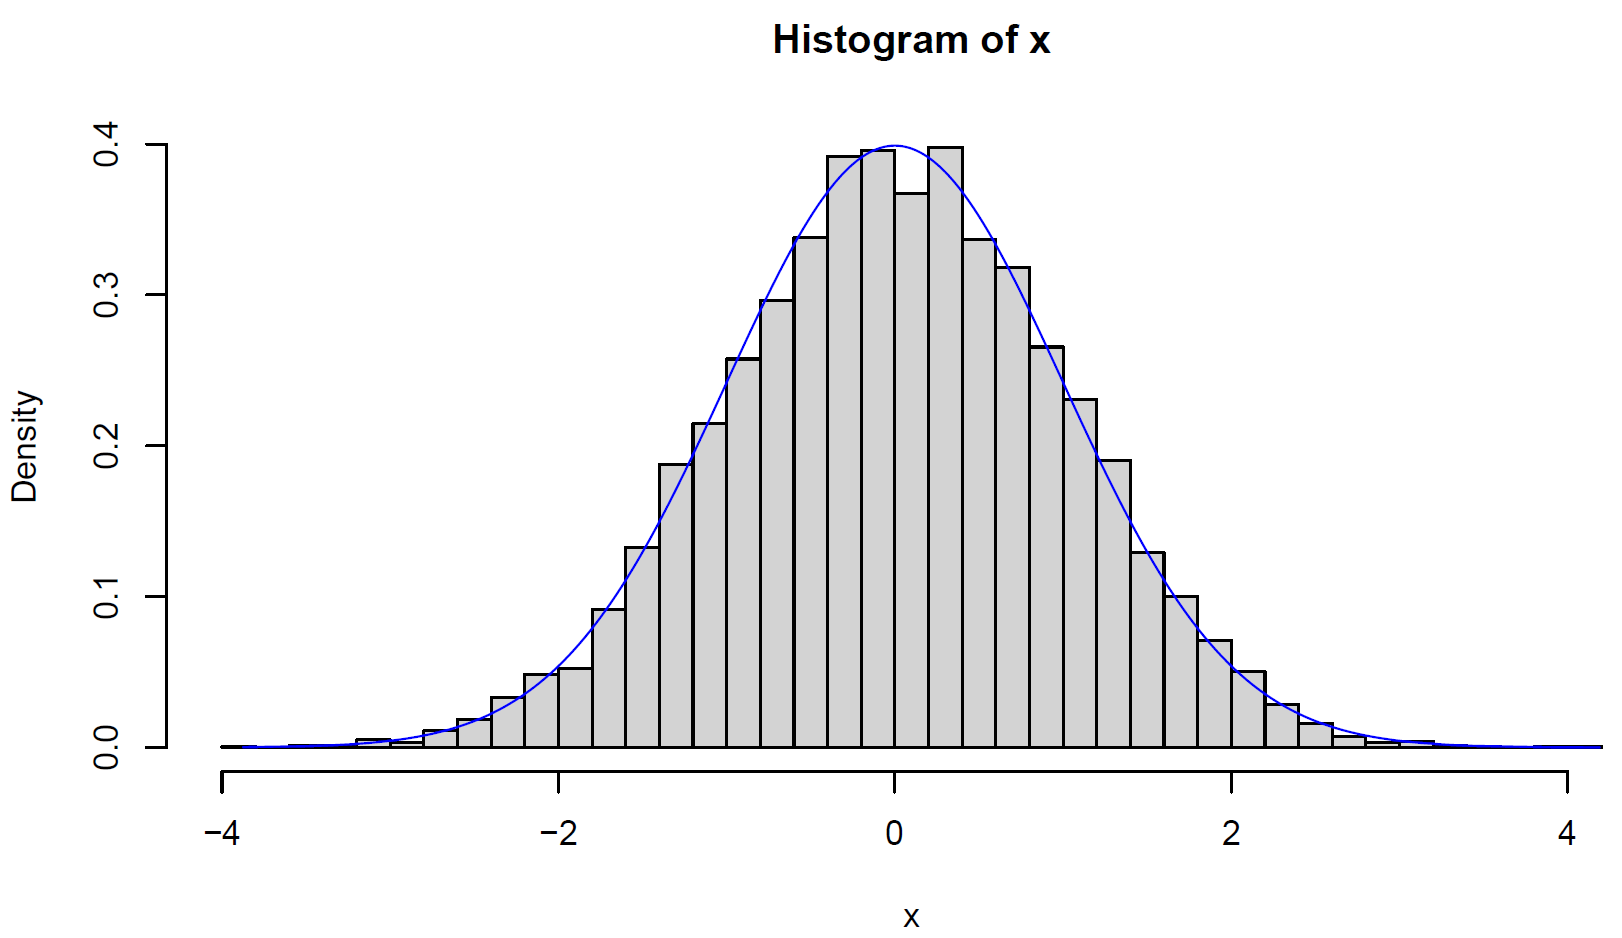
\includegraphics[width =0.9\textwidth]{figure_man/histo.png}
\end{center}

%<<size="scriptsize", echo = FALSE>>=
%rsamp = function(n, dx = dnorm, dy = dcauchy,
%  qy = qcauchy, beta = 0.657) {
%  x = rep(NA, length = n)
%  i = 0
%  while(i < n) {
%    y = qy(runif(1))
%    alpha = beta * dx(y) / dy(y)
%    u = runif(1)
%    if(u <= alpha) {
%      i = i + 1
%      x[i] = y
%    }
%  }
%  return(x)
%}

%set.seed(111)
%x = rsamp(10000)
%hist(x, freq = FALSE, breaks = 50)
%lines(dnorm(x)[order(x)] ~ x[order(x)], col = "blue")
%@
\end{vbframe}


% \begin{vbframe}{Beispiel: Gammaverteilung}
% \begin{center}
%<<include=FALSE>>=
%set.seed(123)
%dx = function(x) dgamma(x, shape = 2)
%dy = function(x) dunif(x, 0, 15)
%qy = function(x) qunif(x, 0, 15)
%x = rsamp(10000, dx = dx, dy = dy, qy = qy, beta = 0.175)
%range(x)
%hist(x, freq = FALSE, breaks = 50,
%  ylim = c(0, 0.4), xlim = c(0, 15))
%lines(dx(x)[order(x)] ~ x[order(x)], col = "blue")
%rect(0, 0, 15, (1 / 15) / 0.175, border = "red", lty = 2)
%@
% \end{center}
% \end{vbframe}


% \begin{vbframe}{Squeezed Rejection Sampling}
% Falls Auswertung von $\alpha(Y) = \beta f_X(Y) / f_Y(Y)$ teuer ist, können obere und untere Schranken $l(Y) \leq \alpha(Y)  \leq  r(Y)$ helfen, falls diese eng und hinreichend einfach zu berechnen sind.
%
% \begin{center}
% <<echo=FALSE, out.width='70%'>>=
% x = seq(-4, 4, length = 101)
% dx = dnorm(x)
% lx = Vectorize(function(val, minx = -2, maxx = 2, h = dnorm(0), m = 0) {
%   if(val < minx | val > maxx) return(0)
%   if(val == m)
%     rval = h
%   else {
%     if(val < m) {
%       b = h / (m - minx)
%       a = 0 - minx * b
%       rval = a + val * b
%     } else {
%       b = h / (m - maxx)
%       a = 0 - maxx * b
%       rval = a + val * b
%     }
%   }
%   rval
% })
% lx2 = function(x) {
%   y = dcauchy(x) / 0.5
%   y[y > dnorm(0)] = dnorm(0)
%   y
% }
% plot(lx(x, -2, 2) ~ x, type = "l", xlim = c(-4, 4), col = "blue", lty = 2,
%   axes = FALSE, ylab = "Density", ylim = c(0, dcauchy(0) / 0.657))
% axis(1)
% axis(2)
% lines(dnorm(x) ~ x)
% lines(lx2(x) ~ x, col = "blue", lty = 2)
% lines(dcauchy(x) / 0.657 ~ x, col = "red", lty = 2)
% @
% \end{center}
%
% \begin{algorithm}[H]
%   \caption{Squeezed Rejection Sampling}
%   \begin{algorithmic}[1]
%   \State{Initialisierung: $f_Y, f_X, N$, linke/rechte Grenzen $l(Y), r(Y)$}
%   \State{$i \leftarrow 0$}
%   \While{$i \ne N$}
%     \State{Erzeuge eine Zufallszahl $Y \sim f_Y$}
%     \State{Erzeuge eine von $Y$ unabhängige Zufallszahl $U$ aus $U[0,1]$}
%     \If{\textcolor{green}{$U \leq l(Y)$} \textcolor{gray}{(anstelle: $U \leq \alpha(Y)$)}}
%       \State{Akkzeptiere $Y$}
%       \State{$i \leftarrow i + 1$}
%     \ElsIf{\textcolor{green}{$U \ge r(Y)$}}
%       \State{Verwerfe $Y$}
%     \EndIf
%   \EndWhile
%   \end{algorithmic}
% \end{algorithm}
%
%
% \begin{itemize}
% \item Ziehe $Y\sim f_Y$ und $U\sim \mathrm \text{U}(0,1)$.
% \item Falls $U \le l(y) \Rightarrow Y$ akzeptieren. \\
% Falls $U \ge r(y) \Rightarrow Y$ verwerfen. \\
% \item sonst:
% \begin{itemize}
% \item Falls $U\le\alpha(Y) \Rightarrow Y$ akzeptieren.
% \item Falls $U > \alpha(Y) \Rightarrow Y$ verwerfen.
% \end{itemize}
% \end{itemize}
%
% \framebreak
%
%
% \end{vbframe}


\begin{vbframe}{Adaptive Rejection Sampling}

Often it is difficult to find a \enquote{good} proposal density $f_Y$. \textbf{Adaptive rejection sampling (ARS)} is an approach to construct adaptive proposal densities. ARS is based on the following ideas:

\begin{itemize}
\item Working with log densities (often algebraically simpler)
\item Use piecewise linear density functions for $f_Y$
\item Adapt $f_Y$ as soon as a proposal $Y$ is rejected
\end{itemize}

\framebreak

\textbf{Procedure:}
\begin{enumerate}
\item Construction of the proposal density $f_Y$
\begin{enumerate}
\item Start with $M := \{y_1,\ldots, y_k\}$
\item Evaluate the log density $l_X := \log f_X(y)$ for all $y \in M$ and find the tangent lines at these points
\item Define a piecewise linear function which is composed of the tangent lines: $l_Y$ $\to$ upper bound for $l_X$


\begin{center}
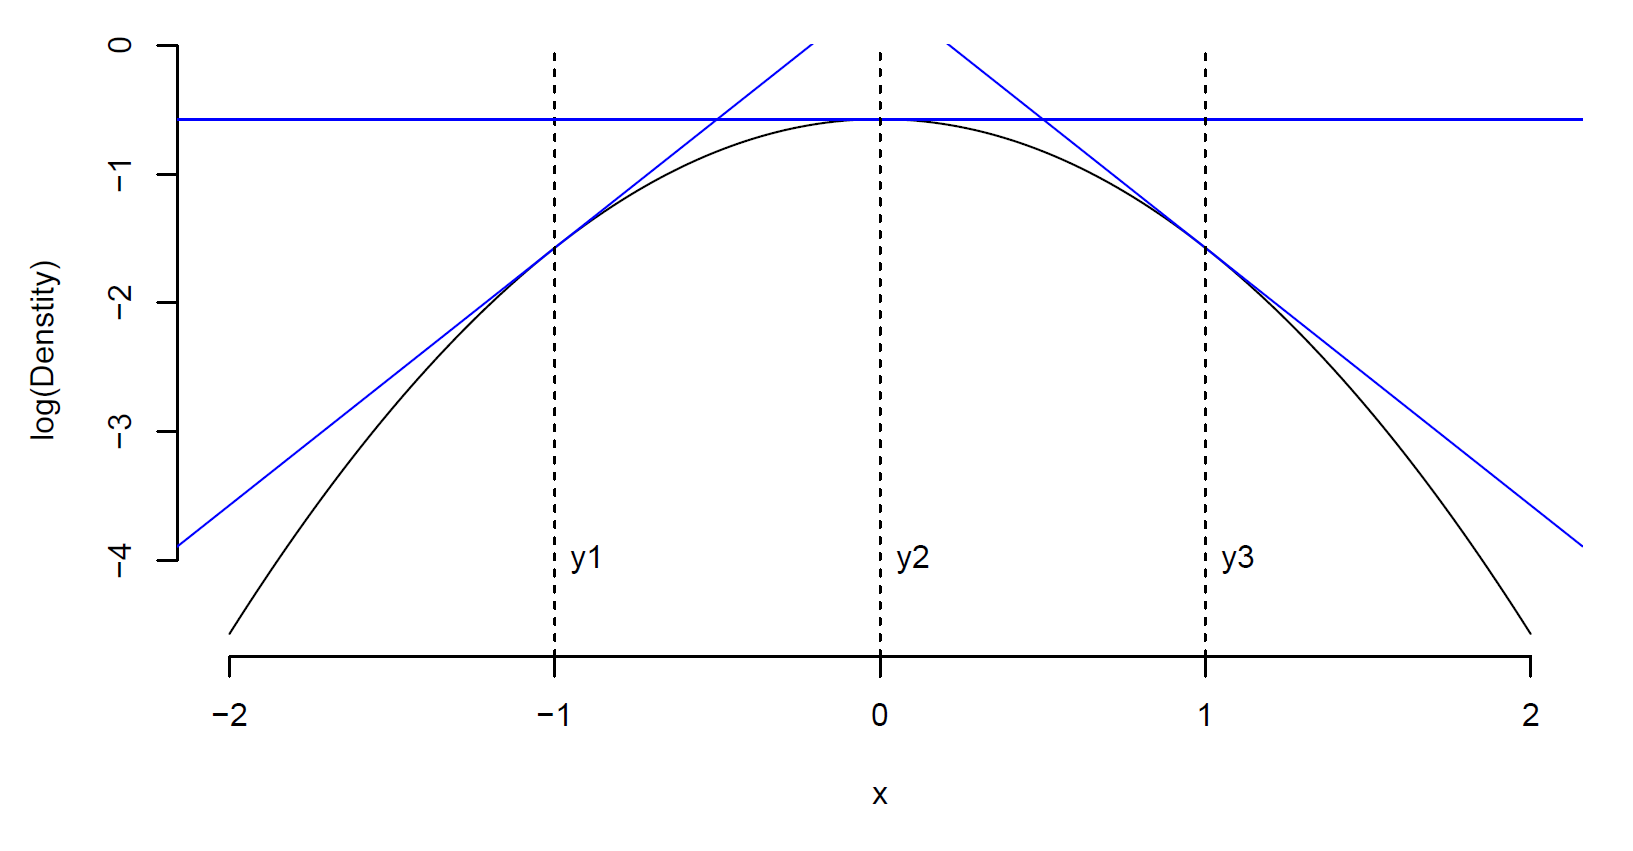
\includegraphics[width =0.4\textwidth]{figure_man/adaptive-rejection.png}
\end{center}

%\setkeys{Gin}{width=1\textwidth}
%<<echo=F, out.width = '60%'>>=
%f = function(x) {
%  1 / 0.03246362 * exp(- 4 - x^2)
%}

%h = function(x) log(f(x))

%dh = function(x) {- 2 * x * f(x) / f(x)}

%x = seq(-2,2,length=1000)
%hmin = min(h(x))

%X = matrix( c( -1, h(-1), 0, h(0), 1, h(1)), nrow = 2)

%x = seq(-2,2,length = 1000)
%plot(x, h(x), type = "l", ylim=c(min(h(x)),max(h(x))+0.4), ylab = "log(Denstity)",
%  axes = FALSE)
%axis(1)
%axis(2)

%for (i in 1:(dim(X)[2])) {
%  x = X[1, i]
%  m = dh(x)
%  y = X[2, i]
%  abline(y - m * x, m, col = "blue")
%  abline(v = x, lty = 2)
%  text(x + 0.1 , -4 , paste("y", i, sep = ""))
%}
%@

\item Back-transform: $f_Y := \exp(l_Y)$

\framebreak


\end{enumerate}
\item \textbf{Rejection sampling:}
\begin{enumerate}
\item Create a random number $Y \sim f_Y$ $^{(*)}$
\item Calculate $ \alpha(Y) = \frac{\exp(l_X(Y))}{exp(l_Y(Y))} = \exp(l_X(Y) - l_Y(Y) )$
\item Create $U \sim \text{U}(0, 1)$
\begin{itemize}
\item If $U \le \alpha(Y)$: Accept $Y$
\item Otherwise: Reject $Y$, add this point to $M$ $\to M \cup Y$ and go to step 1
\end{itemize}

\end{enumerate}
\end{enumerate}

\vfill

\begin{footnotesize}
$^{(*)}$ A method for \enquote{sampling} $f_Y$ and an implementation can be found here: \\
\url{https://blog.inferentialist.com/2016/09/26/adaptive-sampling.html}
\end{footnotesize}

%
%
% Automatische Erzeugung von Hülle und unterer Schranke. %Bedingung: $\log f_X$ ist konkav.
% \begin{itemize}
% \item Untere Schranke: Polygonzug, der Punkte verbindet.
% \item Hülle: Polygonzug aus Tangenten oder Verlängerungen der unteren Schranken.
% \item Updates: setze neue Punkte $x_{k+1}, x_{k+2}, \ldots$ bei
%   akzeptierten Punkten $Y$ (sonst könnte $f_X$ dort klein sein), falls $Y$ über $s(x)$ lag
%   (untere Schranke mit großer Wkt.\ weit von $f_X$ weg).
% \end{itemize}


% \framebreak
%
% \begin{center}
% \end{center}
\end{vbframe}


% \subsection{Ratio of uniforms}
%
%
% \begin{vbframe}{Ratio of uniforms}
% Spezielle Form von Rejection Sampling.\\
% \medskip
% Wenn $(U, V)$ gleichverteilt ist über der Region
% $$
% G_f = \{ (u, v): 0 \leq u \leq \sqrt{f(v / u)} \}
% $$
% für beliebige Funktion $f > 0$, dann hat $X = V / U$ eine Dichte proportional zu $f$.\\
% \medskip
% \textbf{Bemerkung}: Falls $f$ selbst eine Dichte, so gilt $K = \text{area}(G_t) = 1 / 2$.
%
% \framebreak
%
% \begin{center}
% <<echo=FALSE>>=
% a1 = 0
% b1 = 1
% a2 = -sqrt(2 * exp(-1))
% b2 = -a2
% b = tan(seq(-1.57, 1.57, 0.001))
% u = exp(-0.25 * b^2)
% plot(u, b * u, type = "l", xlim = c(a1, b1), ylim = c(a2, b2),
%   xlab = "u", ylab = "v", main = "Ratio of Uniforms N(0, 1)")
% polygon(u, b * u, col = "lightgray")
% @
% \end{center}
%
% \framebreak
%
% \textbf{Beweis}\\
% \medskip
% Sei $K$ die Fläche der Region $G_f$. Dann ist die gemeinsame Dichte von $(U, V)$
% gegeben durch
% $$
% g(u, v) = \begin{cases}
% \frac{1}{K} & \text{für} \quad 0 \leq u \leq \sqrt{f(v / u)} \\
% 0 & \text{sonst.}
% \end{cases}
% $$
% da $(U, V)$ gleichverteilt über $G_f$ sind.\\
% \medskip
% Die Transformation von $(u, v)$ nach $(x, y)$ ist
% $$
% x = \frac{v}{u}, \qquad y = u,
% $$
% d.h.
% $$
% u = y, \qquad v = x \cdot y.
% $$
% Die Jacobi-Matrix der Transformation ist
% $$
% J = \left|
% \begin{array}{cc}
% \frac{\partial u}{\partial x} & \frac{\partial u}{\partial y} \\
% \frac{\partial v}{\partial x} & \frac{\partial v}{\partial y} \\
% \end{array}
% \right| = \left|
% \begin{array}{cc}
% 0 & 1 \\
% y & x
% \end{array}
% \right| = -y.
% $$
% Die gemeinsame Dichte von $X$ und $Y$ ist dann
% $$
% f_{xy}(x, y) = |J|g(y, xy) = \frac{y}{K},
% $$
% für $0 \leq y \leq \sqrt{f(x)}$. Die marginale Dichte von $X$ ist
% $$
% f_{x}(x) = \int\limits_{y = 0}^{\sqrt{f(x)}}f_{xy}(x, y) dy =
%   \int\limits_{y = 0}^{\sqrt{f(x)}} \frac{y}{K}\ dy =
%   \frac{1}{K}\left[ \frac{y^2}{2}\right]_0^{\sqrt{f(x)}} =
%   \frac{1}{2K} f(x).
% $$
% \end{vbframe}
%
%
% \begin{vbframe}{Praktische Anwendung}
% Für praktische Anwendung braucht man Möglichkeit, um von Gleichverteilung auf Gebiet $G_f$ zu ziehen.\\
% \medskip
% Oft schwierig, aber häufig ist $G_f$ beschränkt, liegt also innerhalb von einem Rechteck
% $u \in [0,u_{\text{max}}], v \in [v_{\text{min}},v_{\text{max}}]$.\\
% \medskip
% $\SpAr$ Algorithmus:
% \begin{itemize}
% \item Ziehe $U \sim \text{U}(0,u_{\text{max}})$ und $V\sim \text{U}(v_{\text{min}},v_{\text{max}})$. \\
%   Vorsicht bei Kongruenzgeneratoren auf 2d Eigenschaften!
% \item Berechne $X = V/U$.
% \item Falls $U^2 \leq f(X)$, dann akzeptiere $X$, sonst verwerfen.
% \end{itemize}
% Rejection Sampling für bivariate Gleichverteilung (mehr oder weniger trivial).
%
% \framebreak
%
% <<size="scriptsize">>=
% rusamp = function(n, df = dnorm, range = c(-10, 10)) {
%   tx = seq(range[1], range[2], length = 100)
%   umax = max(sqrt(df(tx)))
%   vmax = max(tx * sqrt(df(tx)))
%   vmin = min(tx * sqrt(df(tx)))
%
%   x = rep(NA, length = n)
%   i = 0
%   while(i < n) {
%     U = runif(1, 0, umax)
%     V = runif(1, vmin, vmax)
%     X = V / U
%     if(U^2 <= df(X)) {
%       i = i + 1
%       x[i] = X
%     }
%   }
%   return(x)
% }
% @
%
% \framebreak
%
% \begin{center}
% <<>>=
% set.seed(123)
% df = function(x) {
%   dgamma(x, shape = 2)
% }
% x = rusamp(10000, df = df)
% hist(x, freq = FALSE, breaks = 50)
% lines(df(x)[order(x)] ~ x[order(x)], col = "blue")
% @
% \end{center}
% \end{vbframe}


\endlecture
\end{document}